\documentclass[tikz,border=14pt]{standalone}
\usepackage{amsmath,amssymb}
\usetikzlibrary{arrows.meta}
\definecolor{ink}{HTML}{E4EDF8}
\definecolor{muted}{HTML}{596B80}
\definecolor{blue}{HTML}{9FC2FF}
\definecolor{teal}{HTML}{63D3BB}
\definecolor{gold}{HTML}{E7C274}
\definecolor{panel}{HTML}{111923}
\pagecolor{panel}
\color{ink}
\begin{document}
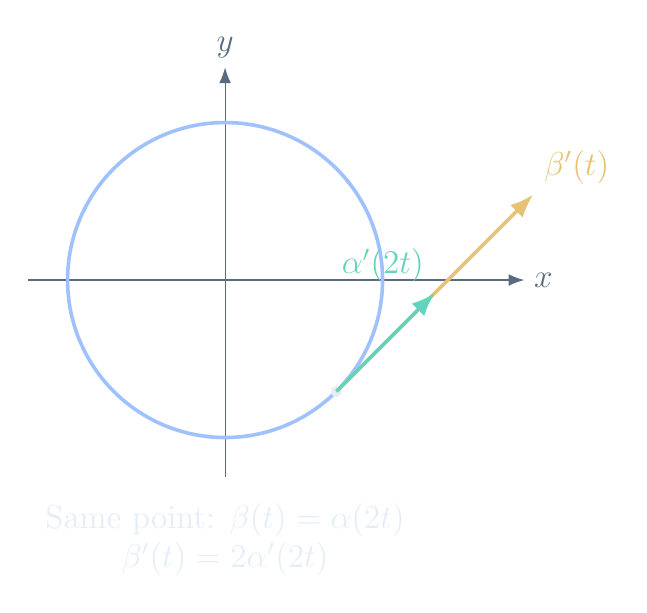
\begin{tikzpicture}[font=\large,text=ink,vec/.style={-{Latex[length=3mm]},line width=1.3pt},axis/.style={muted,-{Latex[length=2mm]},thin}]

\draw[axis] (-2.5,0)--(3.8,0) node[right] {$x$};\draw[axis] (0,-2.5)--(0,2.7) node[above] {$y$};
\draw[blue,line width=1.3pt] (0,0) circle(2);
\coordinate (P) at ({2*cos(-45)},{2*sin(-45)});
\fill[ink] (P) circle(2pt);
\draw[vec,gold] (P)--++(2.5,2.5) node[above right] {$\beta'(t)$};
\draw[vec,teal] (P)--++(1.25,1.25) node[above left] {$\alpha'(2t)$};
\node[align=center] at (0,-3.3) {Same point: $\beta(t)=\alpha(2t)$\\$\beta'(t)=2\alpha'(2t)$};

\end{tikzpicture}
\end{document}
